\documentclass[convert={density=300,outext=.png}]{standalone}
\usepackage{tikz}
\usetikzlibrary{matrix}
\begin{document}
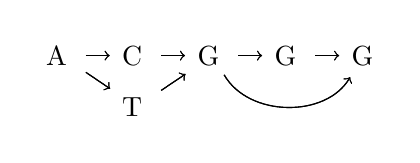
\begin{tikzpicture}[shorten >=1pt,->]
  \def\f{1.2};
  \def\fy{1}

\tikzstyle{vertex}=[circle,fill=black!25,minimum size=17*\f pt,inner sep=0pt]
\matrix (seq) [matrix of math nodes, align=right, row sep=0.5em,column sep=1em, minimum width=1em, minimum height=1em, nodes={align=right}, ]{A & C & G & G & G\\ 
 & T &  &  & \\};
\draw (seq-1-1) -- (seq-1-2);
\draw (seq-1-1) -- (seq-2-2);
\draw (seq-1-2) -- (seq-1-3);
\draw (seq-2-2) -- (seq-1-3);
\draw (seq-1-3) -- (seq-1-4);
\draw (seq-1-4) -- (seq-1-5);
\path [->] (seq-1-3) edge[bend right=60] node {} (seq-1-5);
\draw (seq-1-1) -- (seq-1-2);
\draw (seq-1-1) -- (seq-2-2);
\draw (seq-1-2) -- (seq-1-3);
\draw (seq-2-2) -- (seq-1-3);
\draw (seq-1-3) -- (seq-1-4);
\draw (seq-1-4) -- (seq-1-5);
\path [->] (seq-1-3) edge[bend right=60] node {} (seq-1-5);
\end{tikzpicture}
\end{document}

%%% Local Variables:
%%% mode: latex
%%% TeX-master: t
%%% End:
